\section{烧录}
\subsection{Burning Top-Half}
g-bios上半部分的烧录方法与其他的bootloader一样,都依赖于具体的板子,请大家参考板子的手册烧录TH。
g-bios上半部主要是Load下半部,为下半部服务。Load BH的方式有如下几种:
\begin{enumerate} \setlength{\itemsep}{-\itemsep}
\item 从串口下载下半部并运行
\item 从Flash上Load下半部并运行
\item 自动检测Flash上的下半部是否存在,若存在则默认从Flash上Load下半部并运行,否则等待从串口Load。
\end{enumerate}

\subsection{烧录g-bios BH(下半部分)}
上电或重起后,连接任意键可即可进入g-bios TH的引导菜单。若不按键刚TH默认从Nand Flash中Load BH并执行将执制权交给BH。通过TH Load BH的菜单如下所示:
\begin{figure}[H]
\centering
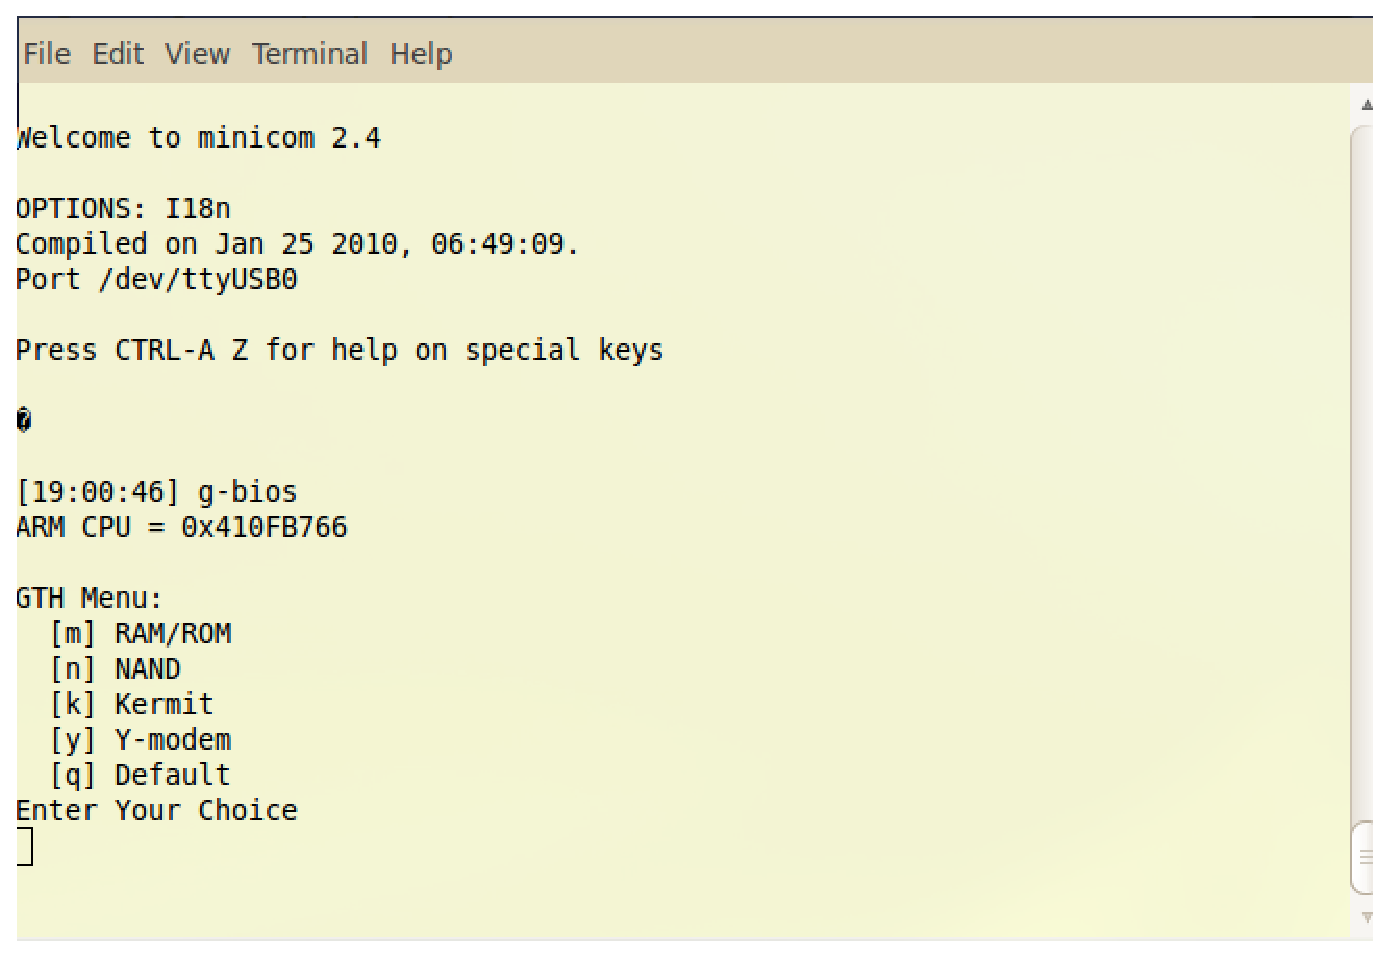
\includegraphics[width=0.8\textwidth]{image/min_01.eps}
\end{figure}
选择不同的选择即可以不同的方式Load BH。以Kermit和Minicom为例从串口引导g-bios bh。
\begin{enumerate} \setlength{\itemsep}{-\itemsep}
\item Ymodem:(注意:minicom在以下过程中要求使用速度很快。)
	\begin{enumerate} \setlength{\itemsep}{-\itemsep}
	\item 连接电源,串口线(开发板上的COM1),网线。
	\item 打开minicom软件。
	\begin{lstlisting}[language=c,numbers=none]
	$ minicom
	\end{lstlisting}
	\item 按下空格键(一直接)。打开电源开关。
	\begin{figure}[H]
	\centering
	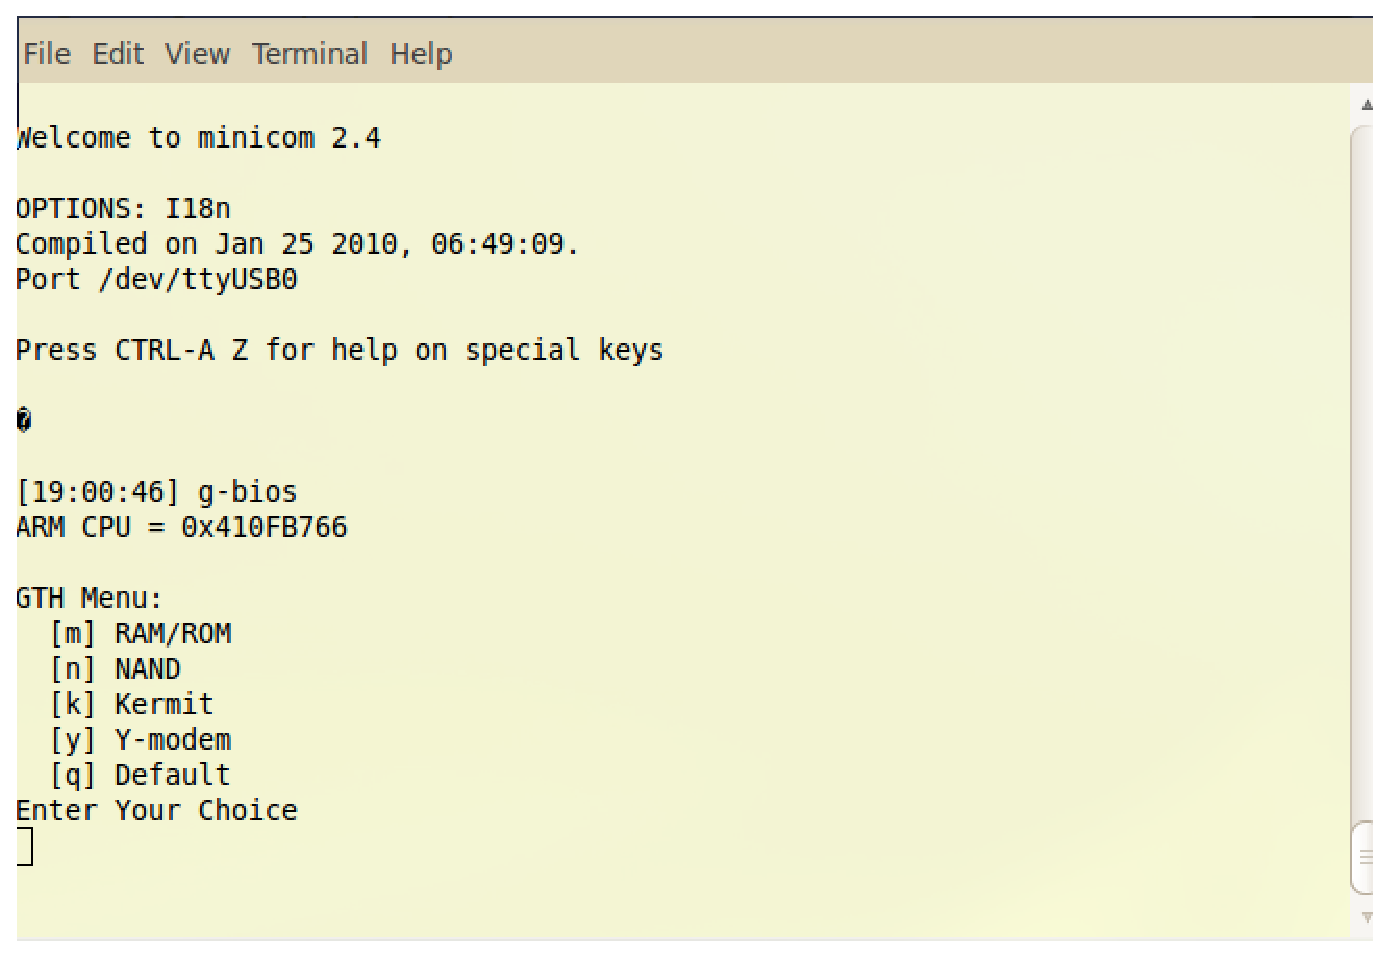
\includegraphics[width=0.8\textwidth]{image/min_01.eps}
	\end{figure}
	\item 按下'Y'键
		\begin{figure}[H]
		\centering
		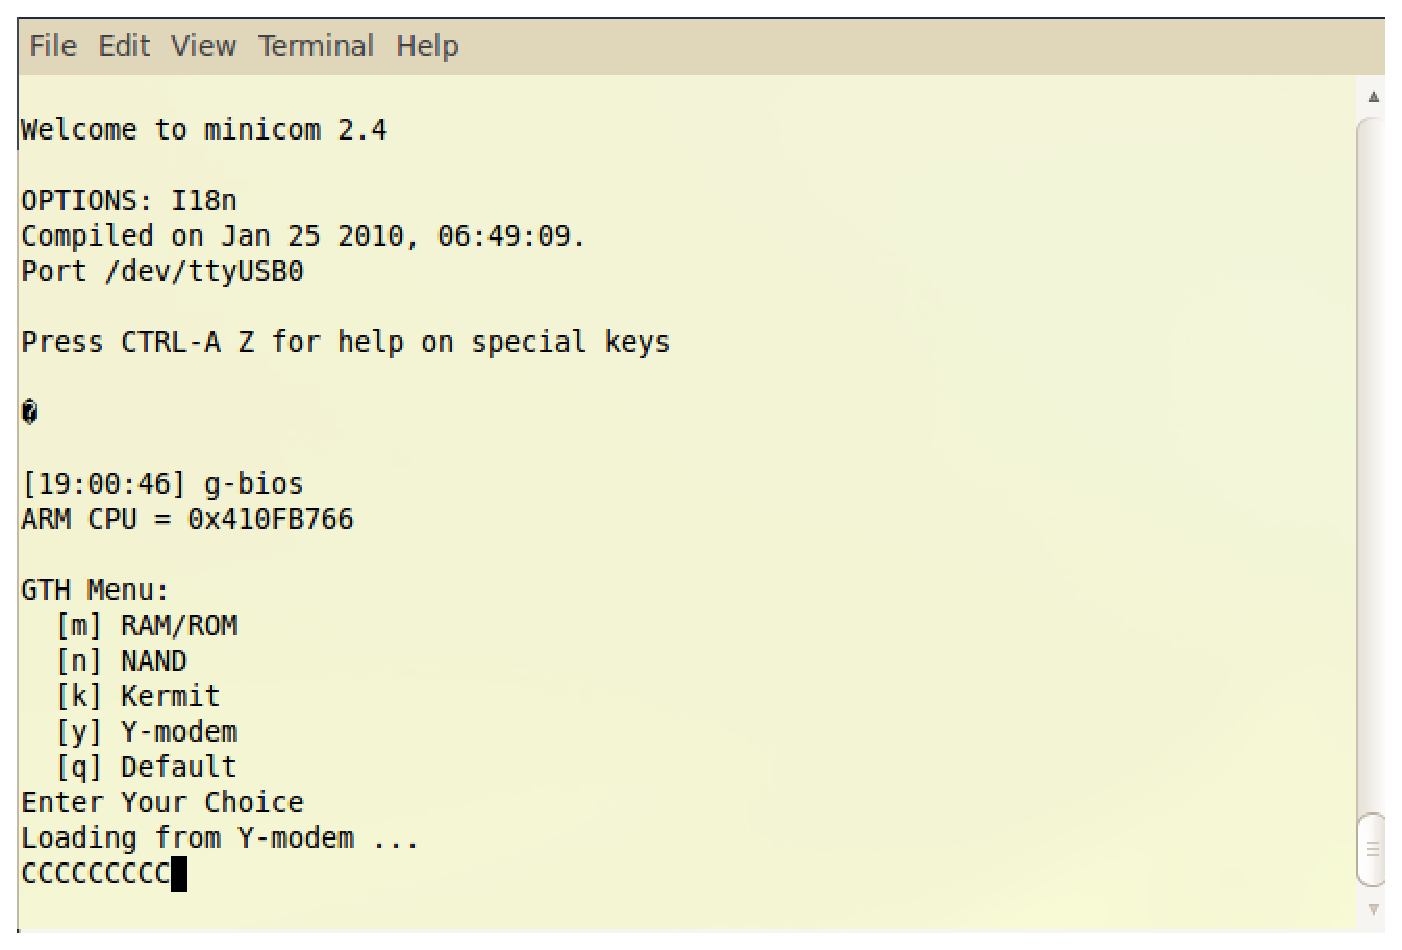
\includegraphics[width=0.8\textwidth]{image/min_02.eps}
		\end{figure}
	\item 同时按下``Ctrl'' + 'a', 再按's'.
		\begin{figure}[H]
		\centering
		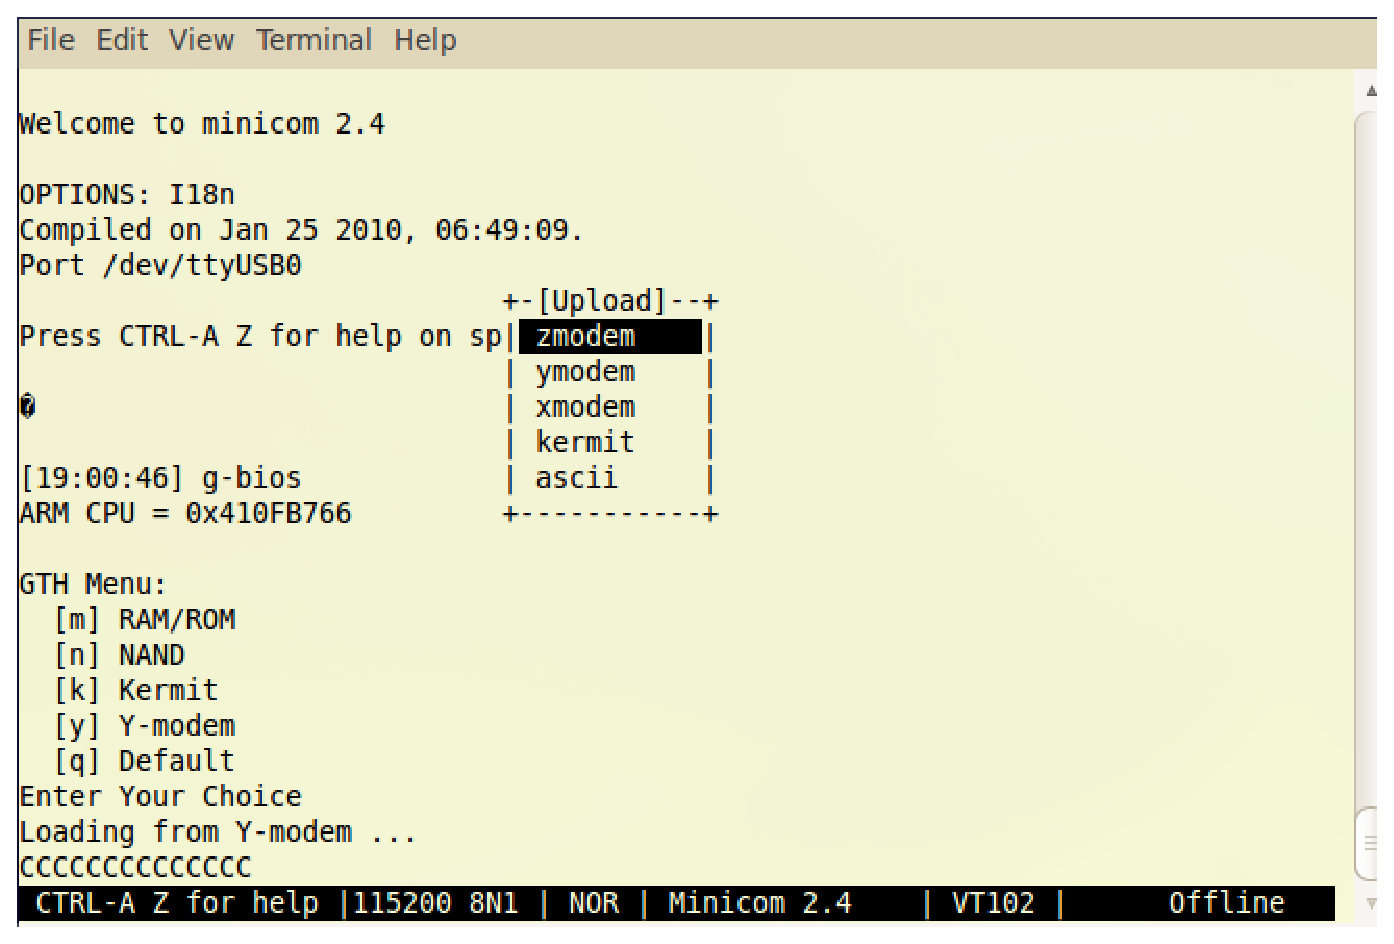
\includegraphics[width=0.8\textwidth]{image/min_03.eps}
		\end{figure}
	\item 用方向键选择``ymodem'',回车。
		\begin{figure}[H]
		\centering
		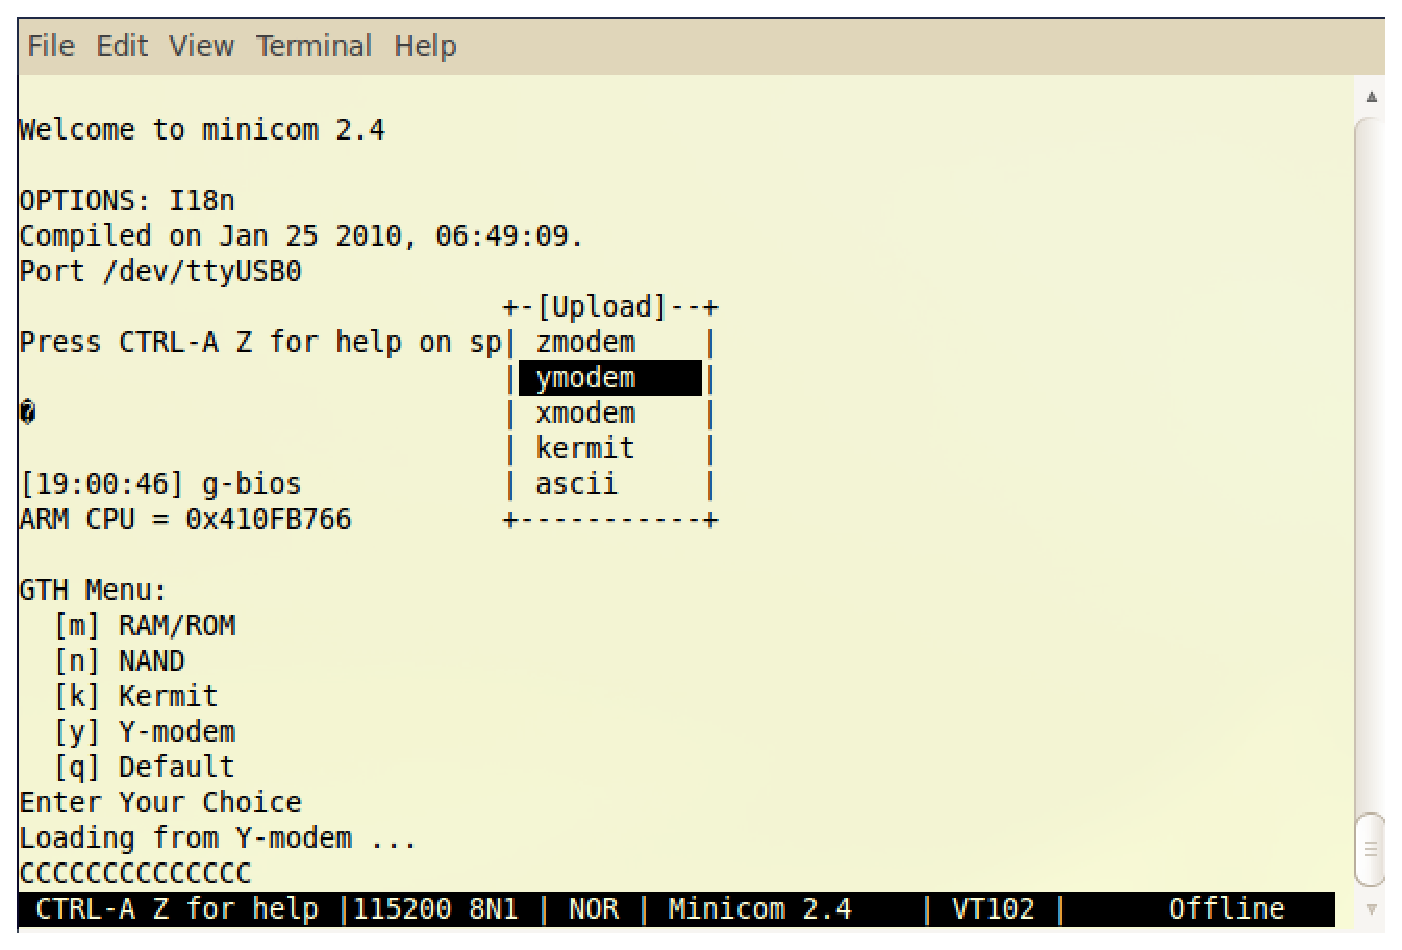
\includegraphics[width=0.8\textwidth]{image/min_04.eps}
		\end{figure}
	\item 选择``Okay'',回车。
		\begin{figure}[H]
		\centering
		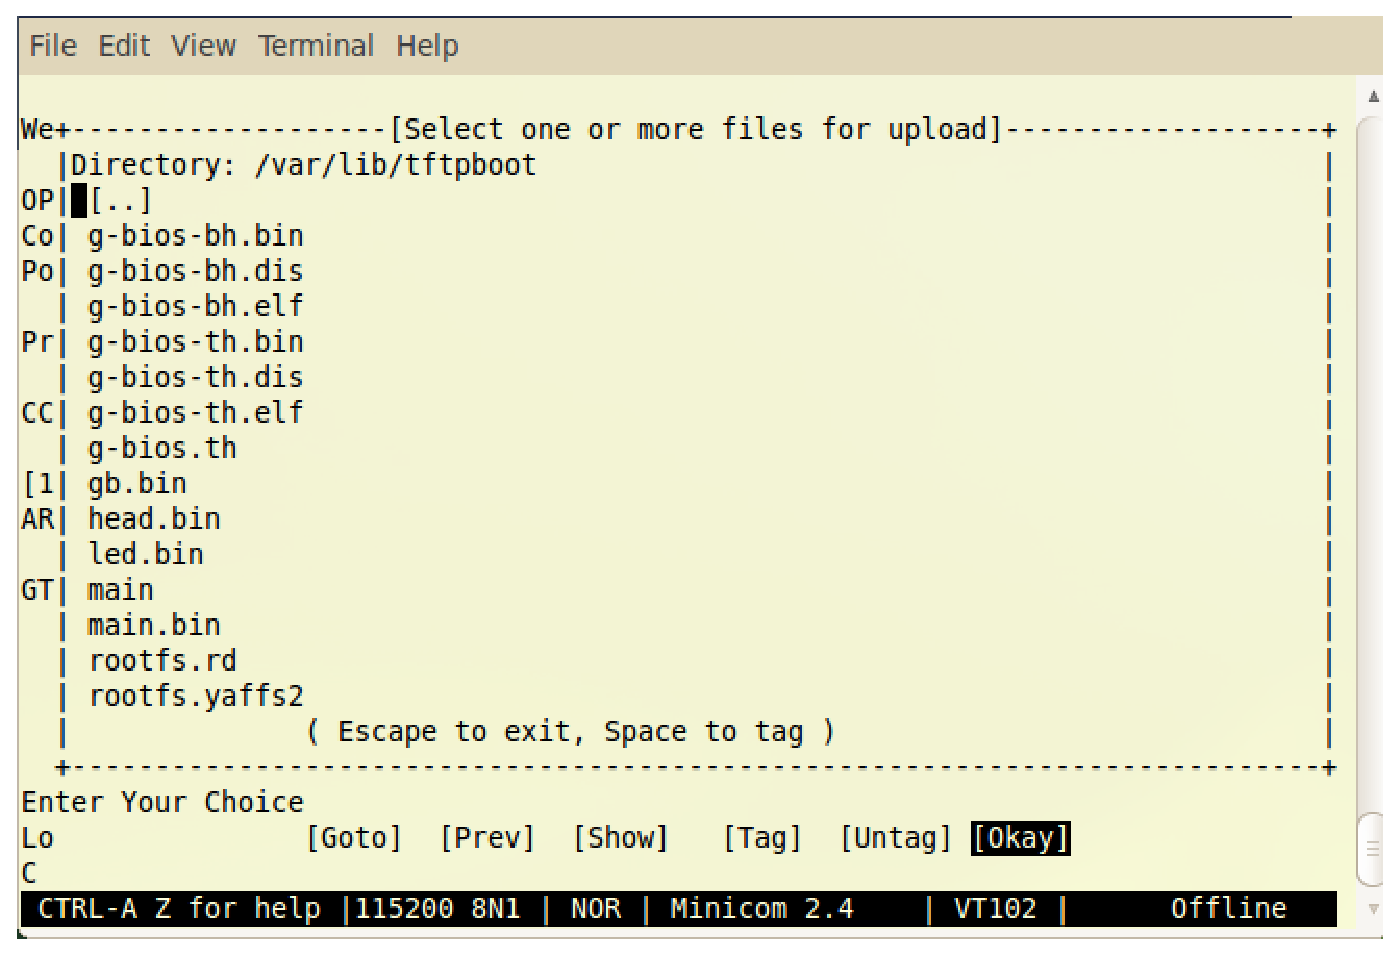
\includegraphics[width=0.8\textwidth]{image/min_05.eps}
		\end{figure}
	\item 输入/var/lib/tftpboot/g-bios-bh.bin。回车。此处输入的为g-bios-bh.bin文件的路径,可视具体情况更改。
		\begin{figure}[H]
		\centering
		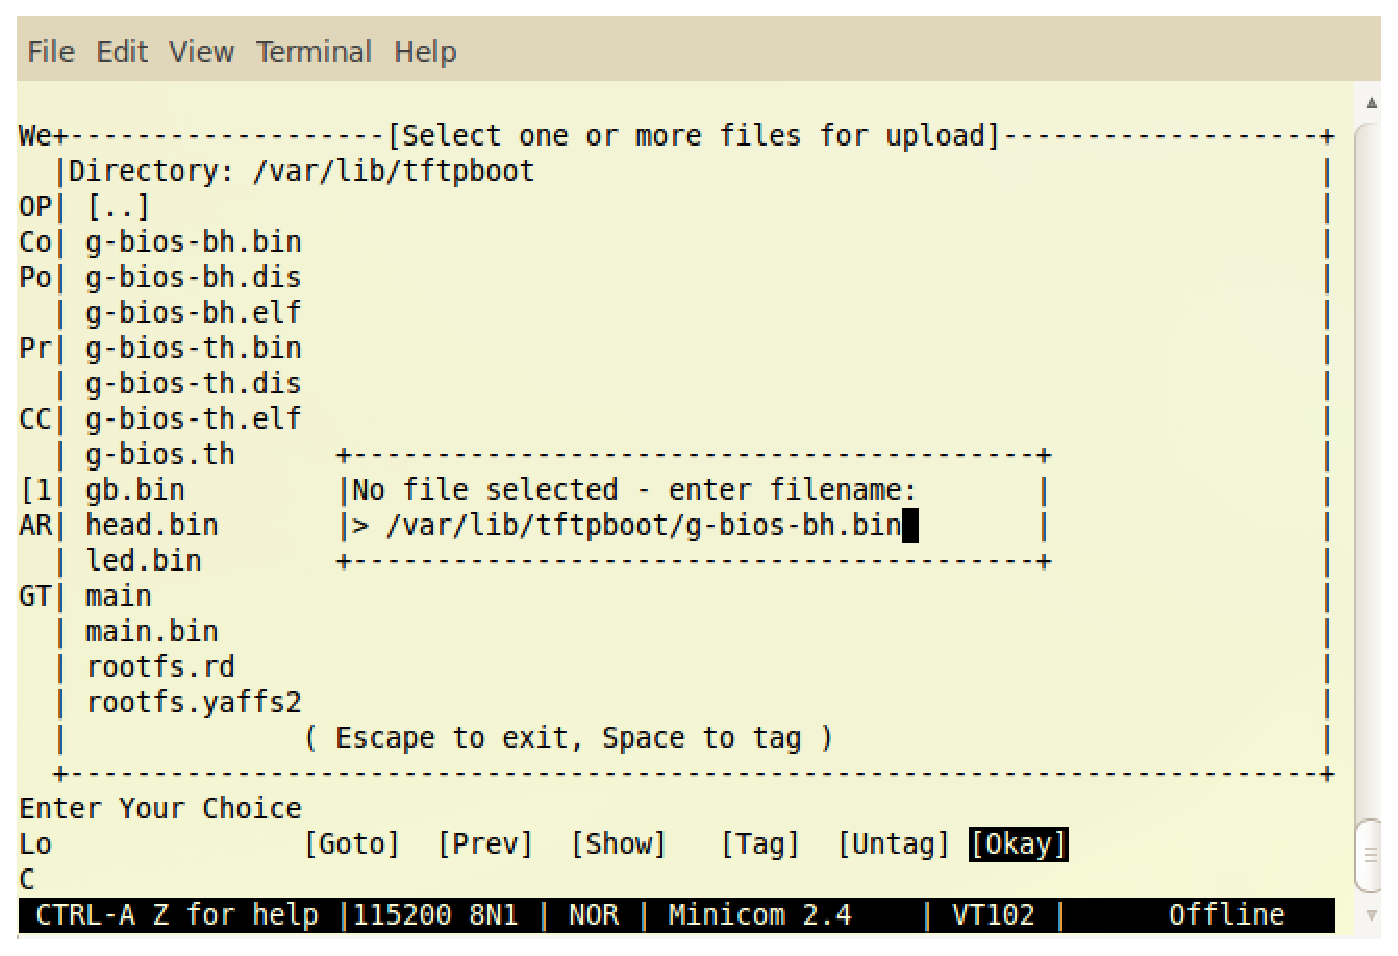
\includegraphics[width=0.8\textwidth]{image/min_06.eps}
		\end{figure}
	\item 开发传输文件,传送完成后如下图所示。再次回车。即可进入g-bios Shell。
		\begin{figure}[H]
		\centering
		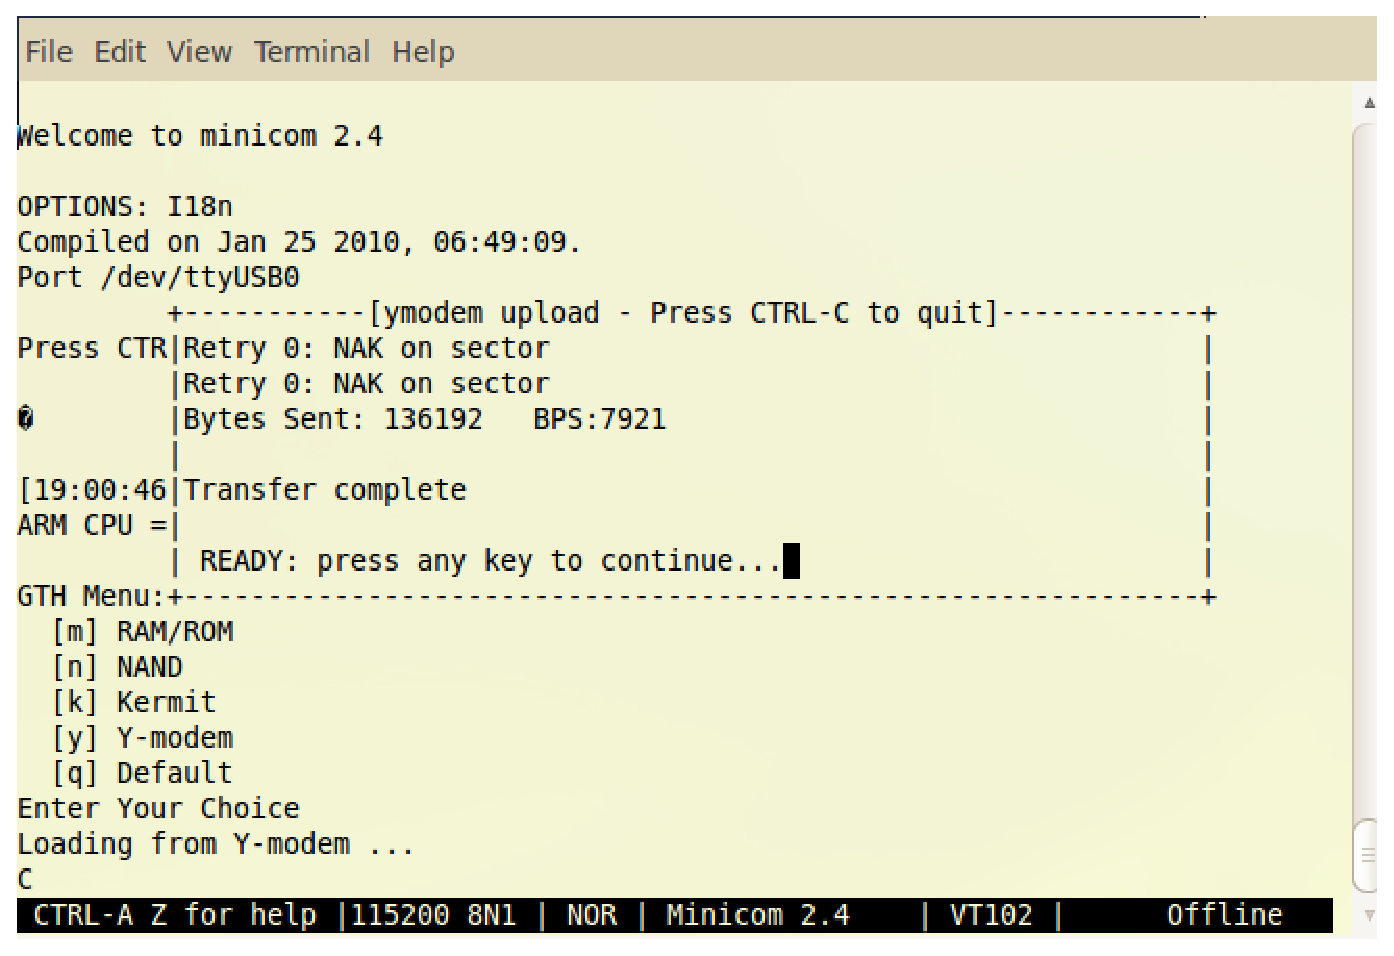
\includegraphics[width=0.8\textwidth]{image/min_07.eps}
		\end{figure}
	\item 进入g-bios Shell。如图所示。
		\begin{figure}[H]
		\centering
		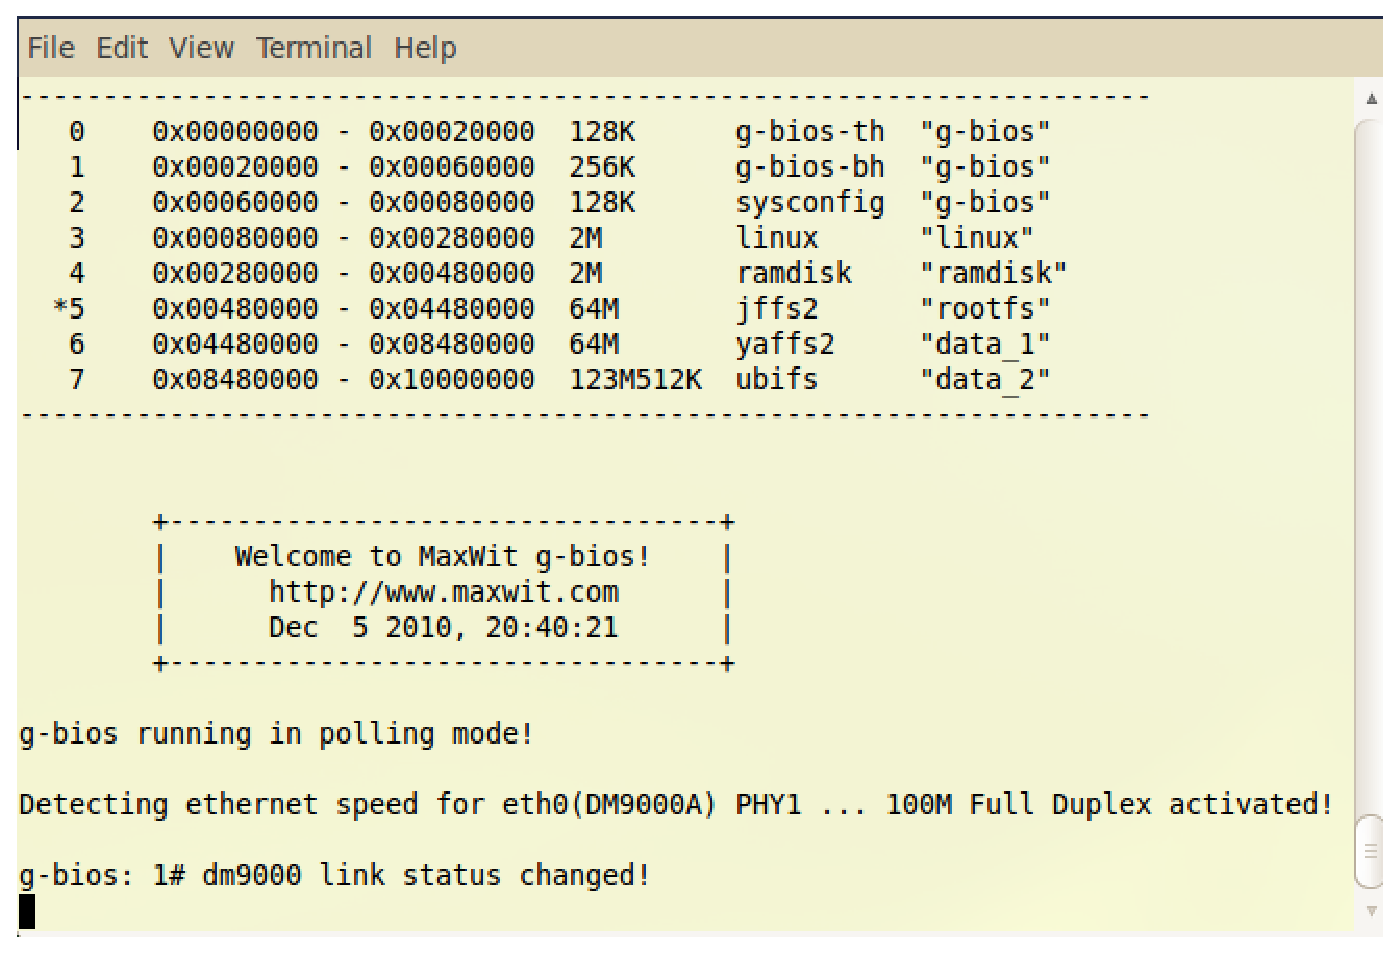
\includegraphics[width=0.8\textwidth]{image/min_08.eps}
		\end{figure}

	如果上述操作失败,以返回第三步(c步)重复操作,在第'f'步,不再重新输入,而是直接回车。
	\end{enumerate}
\item Kermit
\end{enumerate}
\noindent{}第一步,先启动上半部,使用串口线将开发板上的COM1口和PC机的COM口连接、并用网线连接开发板和PC机,在Host端打开kermit\\
\begin{lstlisting}[language=bash,escapeinside=``]
$cd /var/lib/tftpboot
$kermit
C-kermit>c (`回车`)
\end{lstlisting}
\noindent{}第二步,再按下开发板Reset键,将会进入g-bios上半部的启动界面(如图)\\

\begin{figure}[t]
\centering
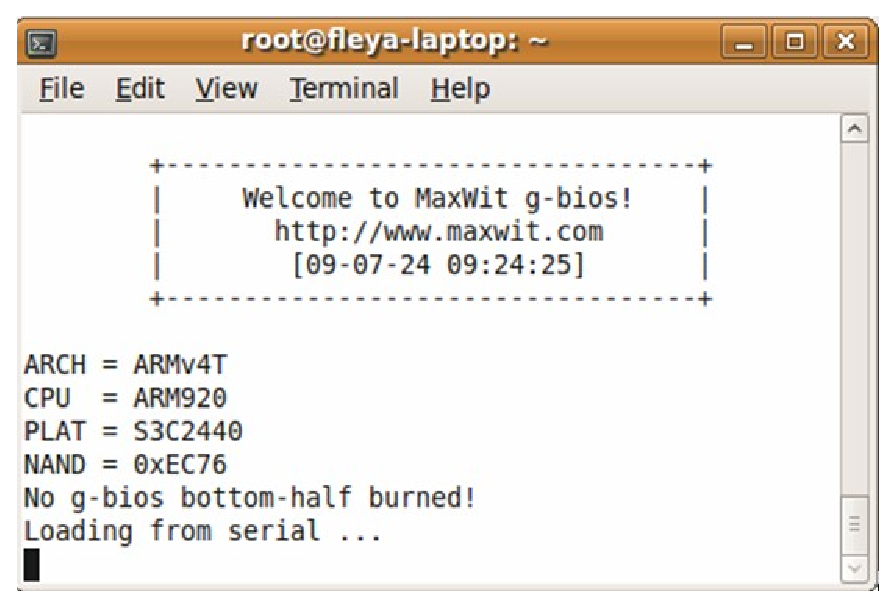
\includegraphics[width=5in]{image/step2.eps}
\end{figure}

\noindent{}注:g-bios的上半部会自动检测Flash上是否已烧录下半部g-bios-bh.bin,若下半部已烧录则直接从Flash上将下半部Load到Sdram并运行,若未烧录则如上图所示,提示下半部未烧录,并需要通过从串口Load下半部并启动。下半部支持通过网络和串口两种方式烧录指定文件到Flash中。也在上半部启动过程中按任意键启动串口Load的功能.

\noindent{}第三步,选择``k''回车, 然后同时按下``CTRL''和``\textbackslash''键, 再按下``c''\\

\begin{figure}[H]
\centering
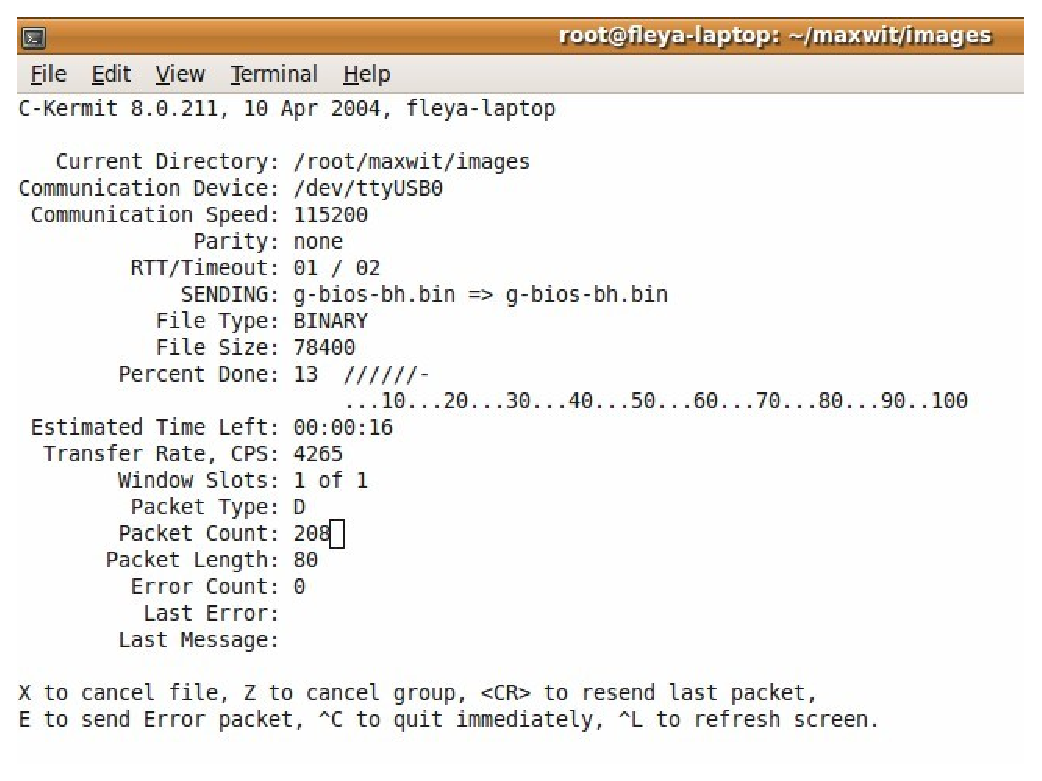
\includegraphics[width=5in]{image/step3.eps}
\end{figure}

\begin{lstlisting}[language=bash,numbers=none]
C-Kermit> send g-bios-bh.bin
\end{lstlisting}
进入g-bios下半部的启动界面,按任意键进入g-bios的命令行,否则g-bios将会自动load kernel并启动(如图)

\begin{figure}[H]
\centering
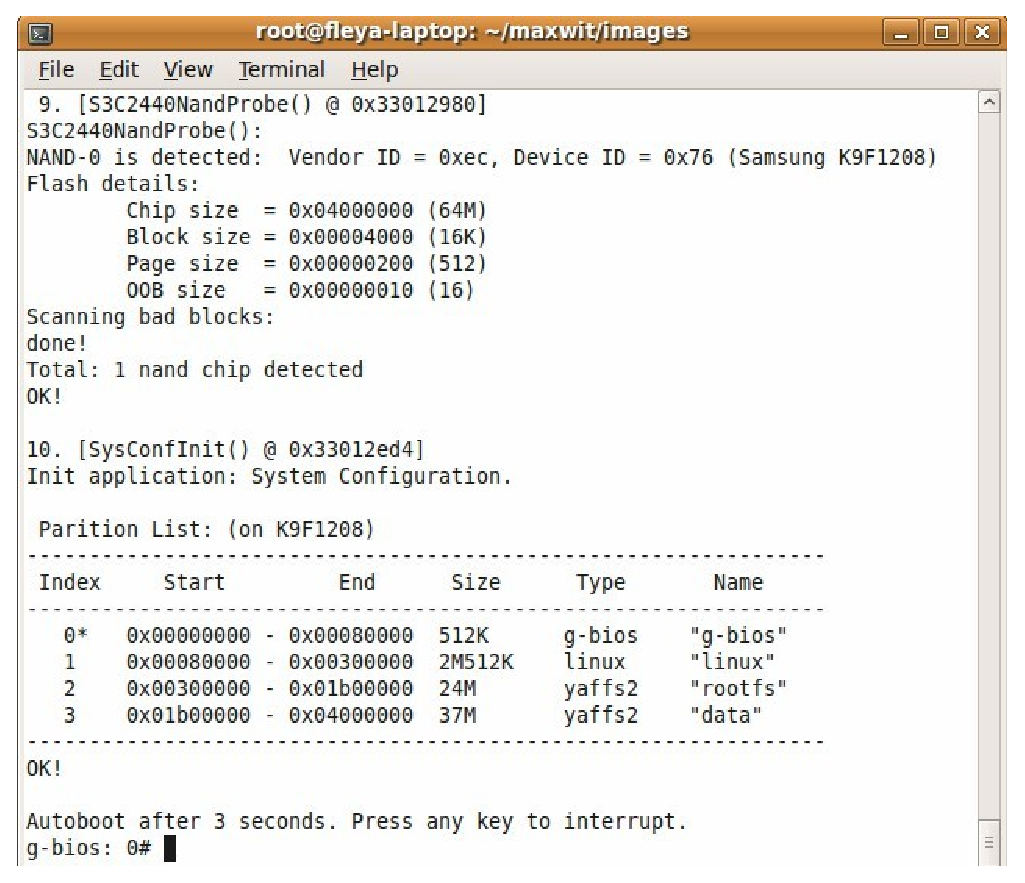
\includegraphics[width=5in]{image/step4.eps}
\end{figure}

\subsection{串口}
\subsection{SD卡}
\subsection{网络}

\begin{enumerate}
\item Write TH Image to SD Card
\item Booting g-bios TH from SD
\item Load BH to RAM
\item Burning TH and BH
\end{enumerate}
